\documentclass[tikz,border=5pt]{standalone}
\usepackage[UTF8]{ctex}
\usepackage{amsmath,amssymb}
\usetikzlibrary{arrows.meta,calc,angles,quotes,decorations.pathmorphing,patterns}
\definecolor{ink}{HTML}{243447}\definecolor{blue}{HTML}{2765A2}
\definecolor{green}{HTML}{3F7D5B}\definecolor{red}{HTML}{B74739}
\tikzset{body/.style={draw=ink,thick},vec/.style={draw=blue,thick,-{Latex}},guide/.style={gray!60,dashed},dim/.style={ink,{Latex}-{Latex}},line cap=round,line join=round}
\begin{document}

\begin{tikzpicture}
\draw[guide](-.4,0)--(5.4,0);
\fill[blue](0,.25)circle(.1)node[above]{$F$};
\fill[red](3.8,.25)circle(.1)node[above]{$C$};
\draw[vec](.2,.25)--(1.65,.25)node[above]{$v_0=0.8c$};
\node[below]at(0,-.2){静质量 $m_0$};
\node[below]at(3.8,-.2){初始静止，静质量 $m_0$};
\draw[vec](4.7,.75)--(5.6,.75)node[right]{$x$};
\node[below]at(2.3,-.85){同一地面参考系；攻击不改变运动者静质量};
\end{tikzpicture}
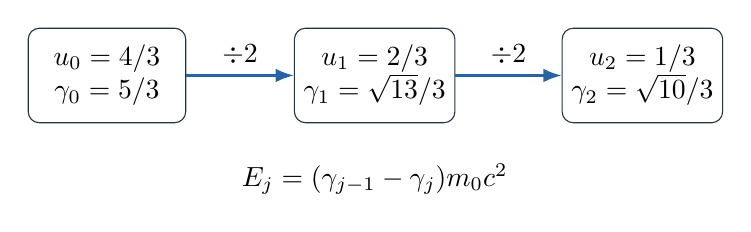
\begin{tikzpicture}
\node[draw=ink,rounded corners,align=center,minimum width=2cm,minimum height=1.2cm](A)at(0,0){$u_0=4/3$\\$\gamma_0=5/3$};
\node[draw=ink,rounded corners,align=center,minimum width=2cm,minimum height=1.2cm](B)at(3.4,0){$u_1=2/3$\\$\gamma_1=\sqrt{13}/3$};
\node[draw=ink,rounded corners,align=center,minimum width=2cm,minimum height=1.2cm](C)at(6.8,0){$u_2=1/3$\\$\gamma_2=\sqrt{10}/3$};
\draw[vec](A)--node[above]{$\div2$}(B);
\draw[vec](B)--node[above]{$\div2$}(C);
\node[below]at(3.4,-1){$E_j=(\gamma_{j-1}-\gamma_j)m_0c^2$};
\end{tikzpicture}
\begin{tikzpicture}
\node[draw=ink,align=center](E)at(0,1){释放能量\\$E_1$};
\node[draw=ink,align=center](K)at(3.5,2){目标动能\\$K_C=E_1/2$};
\node[draw=ink,align=center](R)at(3.5,0){散热辐射\\$E_{\mathrm{rad}}=E_1/2$};
\draw[vec](E.east)--(K.west);
\draw[vec,red](E.east)--(R.west);
\draw[guide](3.5,-.5)--(3.5,-1.3);
\fill[red](3.5,-1.3)circle(2pt);
\draw[vec,red](3.5,-1.3)--(5.4,-1.3)node[above]{$E_+$};
\draw[vec,red](3.5,-1.3)--(1.2,-1.3)node[above]{$E_-$};
\node[below]at(3.3,-1.7){$E_++E_-=E_{\mathrm{rad}},\quad p_{\mathrm{rad}}=(E_+-E_-)/c$};
\node[below]at(3.3,-2.35){本题 $E_->E_+$，净辐射动量向负方向};
\end{tikzpicture}
\end{document}
